% $Id: introduction.tex 34630 2013-04-29 22:53:51Z roldeman $

\section{The Compact Muon Solenoid detector}
\label{sec:CMS}

The Compact Muon Solenoid (CMS) detector is one of two multipurpose detectors built around proton beam collision points at the LHC. In CMS the results of collisions are measured with a series of subdetectors, built within and around a 3.8T superconducting solenoid, designed to track and record the energy of all non-neutrino SM particles \cite{CMSTechDesign1DetectorPerformance}. A representative view of CMS and its components can be seen in Fig.~\ref{fig:CMS}.
\begin{figure}
	\begin{center}
		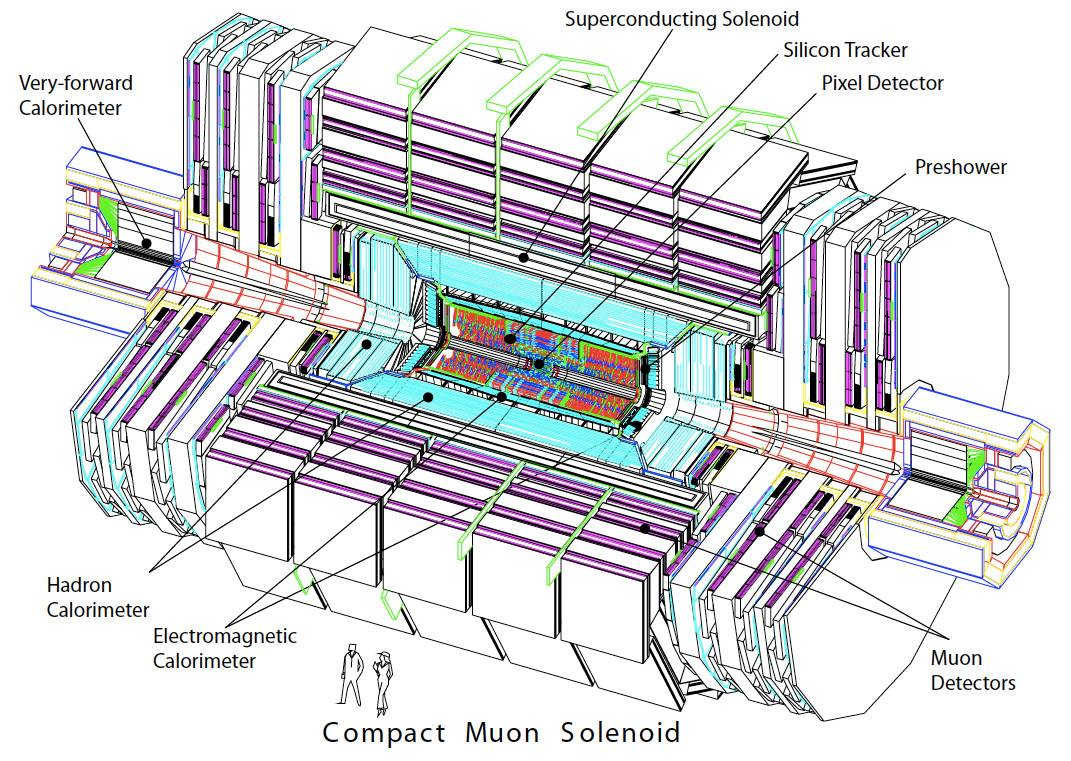
\includegraphics[width=0.8\linewidth]{cms_detector}
	\end{center}
	\caption{An internal view of the Compact Muon Solenoid detector highlighting the key detecting components \cite{CMSTechDesign1DetectorPerformance}}
	\label{fig:CMS}
\end{figure}

\subsection{The Inner Tracking System}
Within the superconducting solenoid is the silicon tracking system that can track \mbox{$p_T>1$~GeV} charged particles with an efficiency greater than $99\%$ \cite{ScienceArticle} \cite{CMSTechDesign1DetectorPerformance}. The Pixel Detector is the high granularity component of the tracking system that sits closest to the interaction point, covering the pseudorapidity region $|\eta|<2.1$ \footnote{$\eta \equiv -ln[tan\frac{\theta}{2}]$, where $\theta$ is measured with respect to the z-axis that points along the beam direction.}. The Silicon Strip Tracker sits around this with barrel and endcap components covering $|\eta|<2.4$. By measuring the curvature of their tracks, charged particle momenta can be measured with an error between $1.5\%$ and $3\%$ for $p_T\sim 100$ GeV \cite{Adam_Elwood_MSci}. The resolution of the trackers is such that the points of origin of event decay products can be inferred within $10$~$\mu$m, allowing the performance of CMS to extend up to very high pileup (number of simultaneous collisions) \cite{CMSTrackPerformance}.

\subsection{The Electromagnetic and Hadronic Calorimeters}
Surrounding the tracking system are the electromagnetic and hadronic calorimeters (ECAL and HCAL). The ECAL is constructed from 75~848 PbWO$_4$ scintillating crystals covering $|\eta|<3$. They are designed to absorb electrons and photons and emit light proportional to the energy deposited. This light is detected by custom photodiodes designed to perform well in high magnetic fields.
\\\\
The HCAL is designed to absorb hadrons and is constructed from brass absorbers interleaved with scintillating plastic tiles covering $|\eta|<3$. The scintillations are read out with hybrid photodiodes via wavelength shifting fibres.
\\\\
In the forward detector regions, the hadronic calorimetry is extended up to $|\eta|<5$ with the Forward Calorimeter, made from steel absorber with quartz scintillating fibre. To also help prevent signal contamination from low energy neutral pions there is a Preshower detector consisting of lead absorbers and silicon microstrips \cite{CMSTechDesign1DetectorPerformance}\cite{Cutajar}.

\subsection{The Muon System}
As muons are unlikely to be absorbed in the ECAL and HCAL, a muon system is built into the iron return yoke that surrounds the solenoid.  This consists of wire chambers containing ionising gas that allows the measurement of muon momenta with a greater than $1\%$ precision \cite{CMS_Overview_Chatrchyan:2008aa}.

\subsection{The Trigger and Data Acquisition System}
The rate of collisions at the LHC is so high that it would be impossible to reconstruct and store the results of all collision events. As the majority of the collisions are soft QCD processes, they are not useful in the search for new physics at the electroweak energy scale. This necessitates a multi-level trigger system that is designed to pick out and store only high centre-of-mass physics processes. The Level 1 Trigger (L1T) is the first component of the trigger system and is made from custom FPGA computational boards situated close to the detector. This uses coarse information from the calorimeters and muon system to reduce the event rate from $20$MHz (during Run 1) to $\sim100$kHz. The data from the subdetectors are then passed to the High Level Trigger (HLT), which uses full detector information to reconstruct the events and reduce the data rate to $\sim1$kHz. The remaining events are then fully reconstructed and stored at various Grid sites \cite{GridTechDesign}.


